% ================================= chapter 3 ================================= %
\chapter{制御系設計}
\subsection{特性解析}
第\ref{chapter_modeling}章で物理パラメータの決定と数式モデルの導出を行った。
ここでは、決定したパラメータから、式(\ref{linear_k}),式(\ref{linear_general})の特性解析を行う。
倒立振子の線形モデルの状態空間表現は以下のようになる。

\begin{equation}
    A,\ B,\ Cの値
    \label{ABC}
\end{equation}

まず、行列$A$の安定判別を行う。$A$のすべての固有値に関して、実部が負であれば$A$は安定性行列である。
すなわち、$A$の固有値$\lambda_{1}$, $\lambda_{2}$, $...$に対し、

$$
    \mbox{Re}[\lambda_{i}] < 0
$$

が成立すればよい。\MaTX{}で$A$の固有値を算出した結果を表\ref{eigen_A}に示す。

\begin{table}[htbp]
    \begin{center}
        \caption{表\ref{eigen_A}: $A$の固有値}
        \begin{tabular}{|c|c|} \hline
            固有値 & Re[$\lambda_{i}$] \\ \hline \hline
            0 & 0 \\ \hline
            0 & 0 \\ \hline
            0 & 0 \\ \hline
            0 & 0 \\ \hline
        \end{tabular}
        \label{eigen_A}
    \end{center}
\end{table}

表\ref{eigen_A}から、倒立振子系のシステムは不安定である。次に、システムの可制御性、可観測性を判別する。
可制御性は、$n$をシステムの次数(倒立振子系のシステムの次数は$n = 4$)に対し、可制御性行列、

$$
    U_{C} =
    \left[
        \begin{array}{ccccc}
            B  &  AB  &  A^2B  &  \dots  &  A^{n-1}B
        \end{array}
    \right]
$$

のランクがシステムの次数と等しければ満たされる。また、可観測性行列は、

$$
    U_{o} = 
    \left[
        \begin{array}{c}
            C \\
            CA \\
            CA^2 \\
            \vdots \\
            CA^{n-1}
        \end{array}
    \right]
$$

であり、$U_{o}$のランクがシステムの次数と等しければ可観測となる。
式(\ref{ABC})において、\MaTX{}を用いて$U_{c}$, $U_{o}$のランクを計算した結果、以下のようになった。

$$
    Uc, Uoのランク
$$

以上から、倒立振子系のシステムは不安定であり、可制御、可観測である。

\subsection{制御システムの構成}
図\ref{controller_system}に、倒立振子系に対する制御システムの構成を示す。

\begin{figure}[htbp]
    \begin{center}
        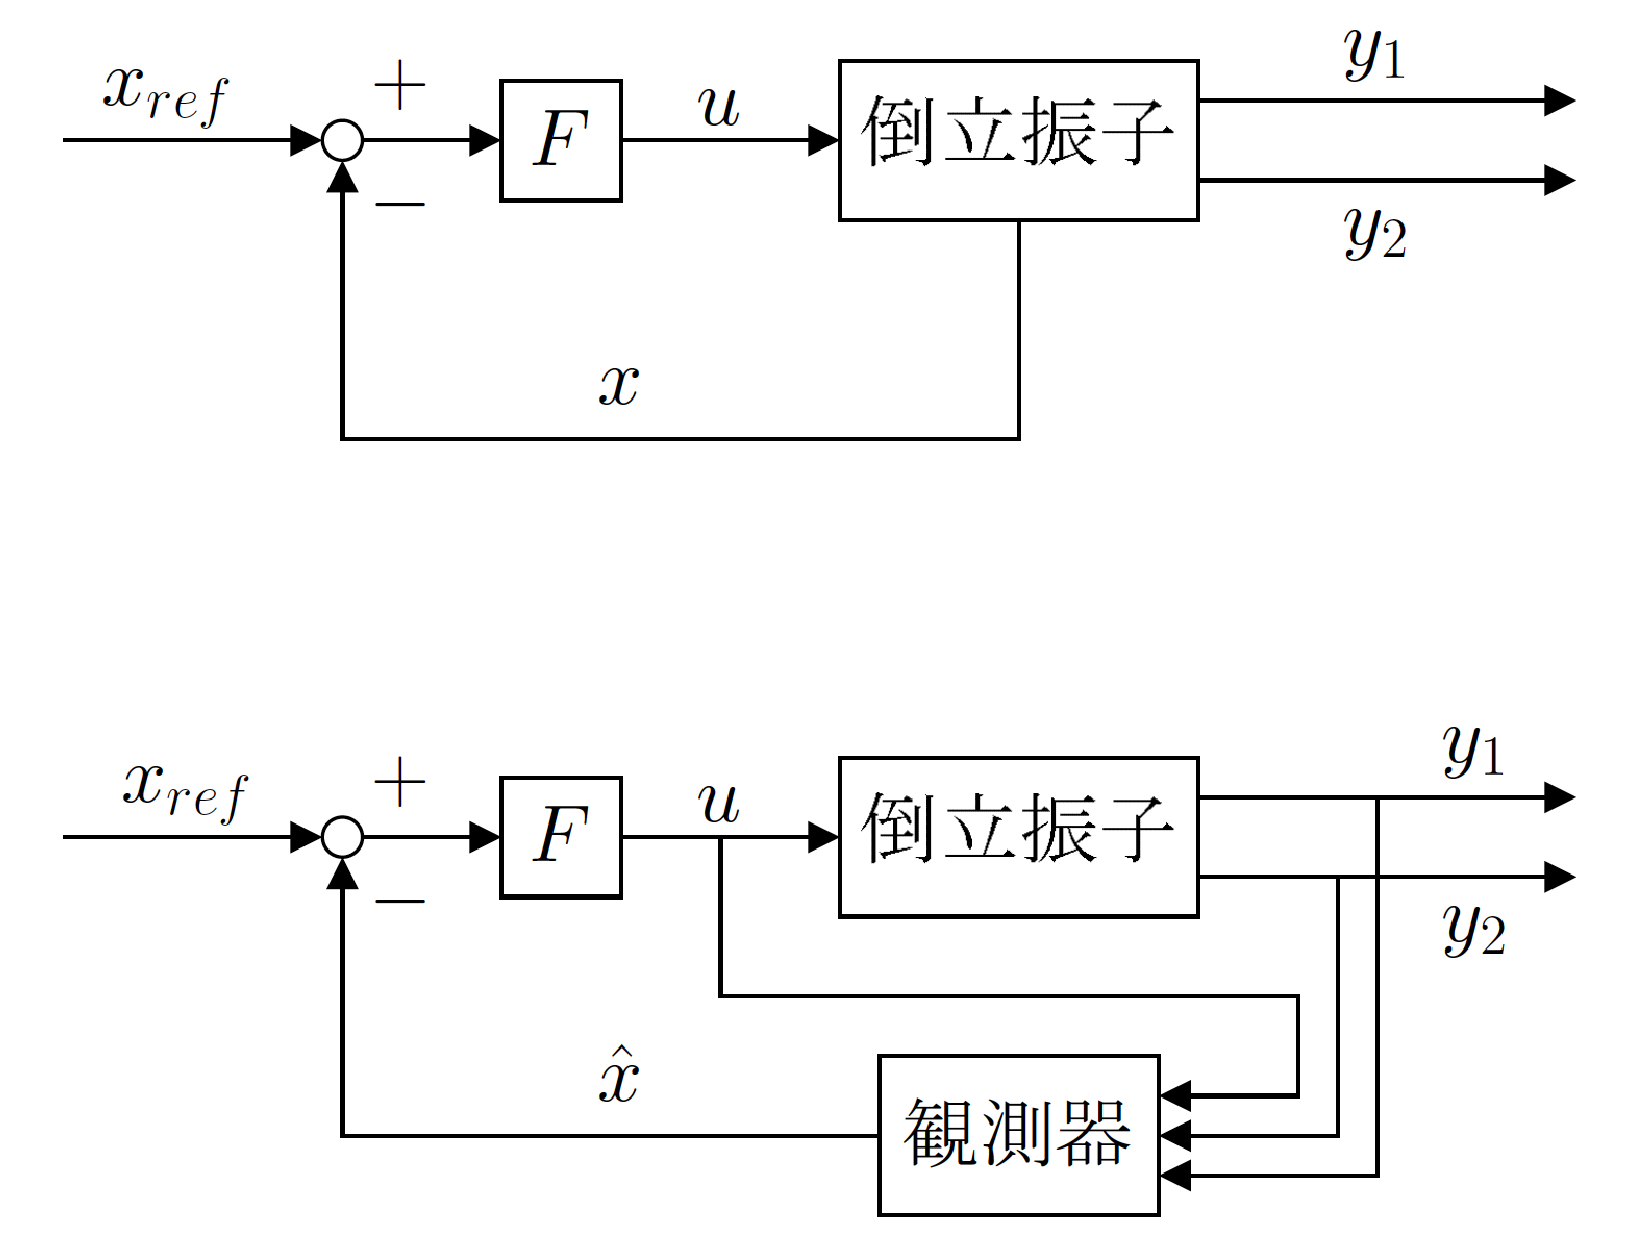
\includegraphics[width=0.6\linewidth]{controller_system.eps}
        \caption{図\ref{controller_system}: 制御システムの構成}
        \label{controller_system}
    \end{center}
\end{figure}

制御系のフィードバックによる入力は、

$$
    u = -F \left( x - x_{ref} \right)
$$

ただし、

$$
    x_{ref} =
    \left[
        \begin{array}{c}
            y_{c} \\
            0 \\
            0 \\
            0
        \end{array}
    \right]
$$

であり、$y_{C}$は指定された台車位置を表す。本実験では、$\dot{r}$, $\dot{\theta}$の検出器は
用いず、状態$x$は推定値$\hat{x}$において、

\begin{equation}
    x = \lim_{t \to \infty} \hat{x}
    \label{definition_x}
\end{equation}

とする。また、式(\ref{definition_x})を満足する最小次元オブザーバ、

\begin{equation}
    \hat{z} = \hat{A}z + \hat{B}y + \hat{J}u
    \label{z_hat}
\end{equation}

\begin{equation}
    \hat{x} = \hat{C}z + \hat{D}y
    \label{x_hat}
\end{equation}

を用いる。ここで、オブザーバの次数は$2$であり、設計すべき制御システムは以下のようになる。

\begin{itemize}
    \item $F(1 \times 4)$
    \item $\hat{A}(2 \times 2)$, $\hat{B}(2 \times 2)$, 
    $\hat{J}(2 \times 1)$, $\hat{C}(4 \times 2)$, $\hat{D}(4 \times 2)$
\end{itemize}


\subsection{状態フィードバック$F$の設計}
$F$は、システムを安定化する状態フィードバック、

\begin{equation}
    u = -Fx
    \label{feedback_u}
\end{equation}

を満たすように求める。式(\ref{feedback_u})をLQ問題として解くため、$2$次形式評価関数、

\begin{equation}
    J = \int_{0}^{\infty}
    \left(
        x^{T}Qx + Ru^2
    \right)
    dt
    \label{eval2_J}
\end{equation}

\begin{equation}
    Q = \mbox{diag}(q_{1}^2, q_{2}^2, q_{3}^2, q_{4}^2), R = 1
    \label{eval2_Q}
\end{equation}

を考える。ここで、$\mbox{diag}(\dots)$は、各引数を固有値にもつ対角行列を表す。これは、

\begin{equation}
    J = \int_{0}^{\infty}
    \left(
        q_{1}^2 r^2 + q_{2}^2 \theta^2 + q_{3}^2 \dot{r}^2 + q_{4}^2 \dot{\theta}^2 + u^2
    \right)
    dt
\end{equation}

と表せるから、$q_{1}$, $q_{2}$, $q_{3}$, $q_{4}$はそれぞれ、台車位置$r$, 振子角度$\theta$,
台車速度$\dot{r}$, 振子角速度$\dot{\theta}$に対する重み係数である。
式(\ref{eval2_J}), 式(\ref{eval2_Q})を最小にする$F$は、リッカチ方程式、

$$
    A^{T}P + PA - PBR^{-1}B^{T}P + Q = 0
$$

の解$(P > 0)$に対し、

$$
    F = R^{-1}B^{T}P
$$

で与えられる。

\subsection{$\hat{A}$, $\hat{B}$, $\hat{C}$, $\hat{D}$, $\hat{J}$の設計}
式(\ref{z_hat}), 式(\ref{x_hat})が式(\ref{definition_x})を満足するための十分条件は、
ある行列$U(1 \times 4)$が存在して、

$$
    \begin{array}{c}
        UA = \hat{A}U + \hat{B}C \\
        UB = \hat{J} \\
        I = \hat{C}U + \hat{D}C
    \end{array}
$$

であり、かつ$\hat{A}$が安定性行列であることである。これらの条件を満足するオブザーバを設計するため、
Gopinathの方法を用いる。

\subsection{制御システムの離散化}
式(\ref{feedback_u}), 式(\ref{z_hat}), 式(\ref{x_hat})で示した$u,\ \hat{z},\ \hat{x}$は、
連続時間上で設計される制御器である。そこで、計算機で制御器を表現するためこれらの離散時間化を行う。
各サンプリングの間隔を$\Delta$とすると、

$$
    \begin{array}{c}
        u[k] = -F \hat{x}[k] \\
        z[k + 1] = \hat{A}_{d}z[k] + \hat{B}_{d}y[k] + \hat{J}_{d}u[k] \\
        \hat{x}[k] = \hat{C}_{d}z[k] + \hat{D}_{d}y[k]
    \end{array}
$$

と表せる。ただし、$k = 0, 1, \dots$において、

$$
    x_{ref} = 
    \left[
        \begin{array}{cc}
            \hat{A}_{d}  &  \left[
                                \begin{array}{cc}
                                    \hat{B}_{d}  &  \hat{J}_{d}
                                \end{array}
                            \right] \\
            0            &  I_{3}
        \end{array}
    \right]
    =
    \exp \Delta
    \left[
        \begin{array}{cc}
            \hat{A}  &  \left[
                            \begin{array}{cc}
                                \hat{B}  &  \hat{J}
                            \end{array}
                        \right] \\
            0        &  I_{3}
        \end{array}
    \right]
$$

である。

\subsection{振り上げ制御と安定化}



% =============================== chapter 3 END =============================== %